\documentclass{standalone}
\usepackage{tikz}

\begin{document}

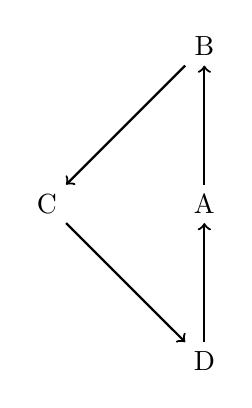
\begin{tikzpicture}
    % Define four nodes arranged in a circle (90 degrees apart)
    \node (A) at (0,0) {A};
    \node (B) at (90:2cm) {B};
    \node (C) at (180:2cm) {C};
    \node (D) at (270:2cm) {D};
    
    % Draw directed arrows from each node to the next clockwise
    \draw[->, thick] (A) -- (B);
    \draw[->, thick] (B) -- (C);
    \draw[->, thick] (C) -- (D);
    \draw[->, thick] (D) -- (A);
\end{tikzpicture}

\end{document}